\chapter[Gerência de requisitos]{Gerência de requisitos}

Nessa seção será definido os atributos que os requisitos conterão a fim de permitir sua gerência. Assim como descrever os relacionamentos existente entre eles e possibilitar a sua rastreabilidade, analisar possíveis impactos  caso sejam alterados.

No processo de engenharia de requisitos de software é necessário controlar as mudanças que ocorrem nos requisitos, a atividade responsável por isto é a gerência de requisitos.

Dentre as mudanças têm-se, de acordo com \cite{silva2011}:
\begin{itemize}
    \item Melhor compreensão das necessidades do sistema pelos stakeholders;
    \item Descoberta de novos requisitos;
    \item Feedback das atividades já desenvolvidas propiciando mudanças;
\end{itemize}

Cada mudança dessa tem um impacto no desenvolvimento do projeto e é competência da atividade de gerência de requisitos controlar essas mudanças de forma que seja mensurável o impacto delas, os riscos associados, as alterações no cronograma e orçamento de um projeto.\cite{silva2011}

\section{Rastreabilidade de requisitos}

Com as mudanças constantes no desenvolvimento, é preciso reconhecer quais requisitos mudaram, quais os outros requisitos serão afetados por essa mudança. Assim, a rastreabilidade de requisitos provem os relacionamentos entre os requisitos \cite{leite2005}.

Deve-se atribuir identificadores únicos aos requisitos para que possa rastreá-los, e além disso, identificar as relações entre os artefatos produzidos no processo de desenvolvimento, qual o requisito de origem possibilitou em um alguma implementação \cite{silva2011}.

Há dois tipos de de rastreabilidade:
\begin{itemize}
    \item \textbf{Pré-rastreabilidade:} relacionamento bi-direcional no qual permite que os interesses do cliente possam ser localizados nos requisitos \cite{silva2011}.
    \item \textbf{Pós-rastreablidade:} é a conexão bi-direcional em que possibilita identificar os requisitos que originaram as implementações \cite{silva2011}.
\end{itemize}

Os requisitos estão envolvidos por um elo de ligação, o modelo de Ramesh e Jarke definem que este elo pode ser agrupado pela categoria relacionados ao produto. Este define duas propriedades dos relacionamentos que são: Elos de satisfação e de dependência \cite{leite2005}.

Os elos de satisfação garantem que os requisitos estejam relacionados a algum componente do sistema e assim todo componente possui no mínimo um requisito associado a ele. Já os elos de dependência auxiliam o gerenciamento das dependências de recursos e compatibilidades, ou seja, possibilitam criar uma associação de dependência entre requisitos e recursos, isto auxilia o controle de impacto nas alterações de um artefato, e nos artefatos que dependem dele \cite{leite2005}.

O projeto adota as metodologias ágeis para o desenvolvimento das atividades, o scalade agile framework fornece um modelo abstrato dos requisitos \cite{safe}. Na figura é possível ver os níveis de requisitos e sua rastreabilidade da forma Epic > Features > Story. Vale notar que há mais um nível descrito, capabilities. Este nível de representação de requisito é utilizado no nível Value Stream definido pelo SAFe 4 níveis, este nível é direcionado a projetos maiores e mais complexos, que geralmente possuem multidisciplinaridade, e que portanto não é aplicável ao contexto deste projeto.

\begin{figure}[H]
    \centering
    \caption[Modelo de requisitos]{Modelo de requisitos. fonte:\url{http://www.scaledagileframework.com/safe-requirements-model/}}
    \label{modeloRequisitos}
    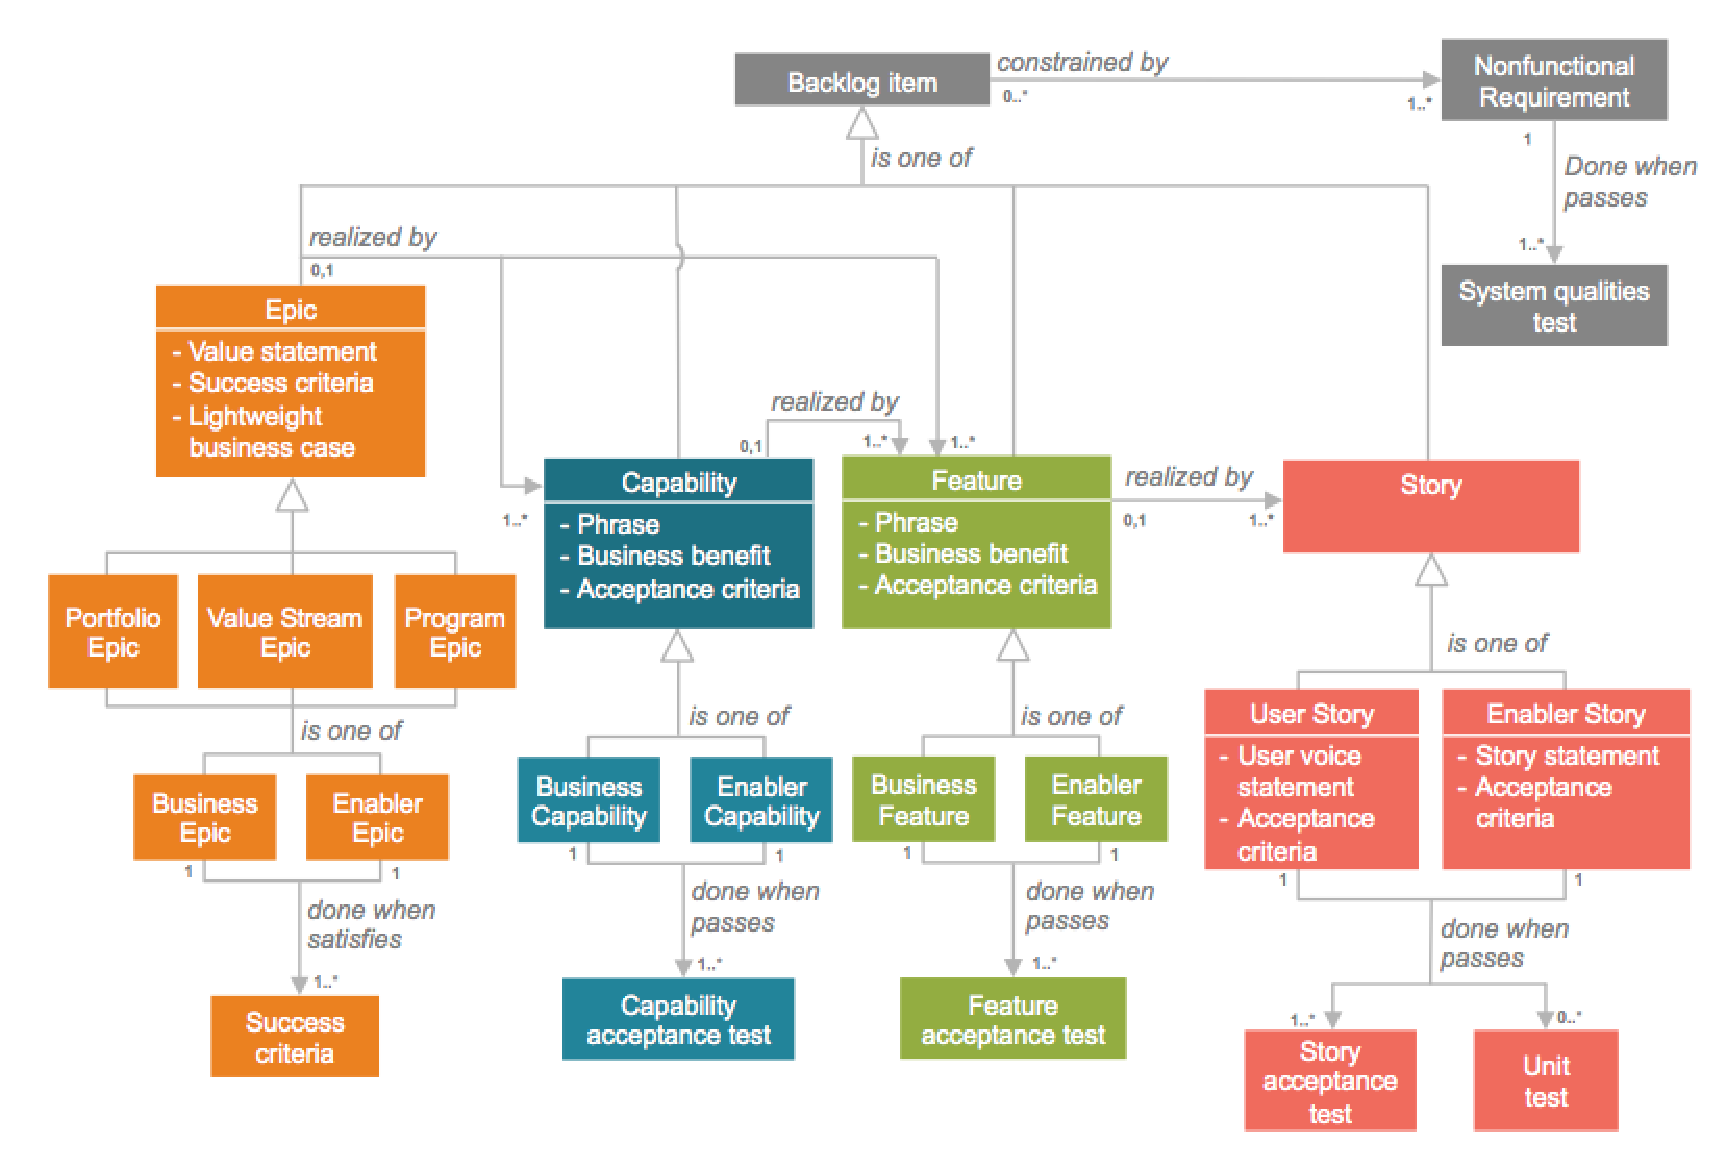
\includegraphics[keepaspectratio=true,scale=0.5]{figuras/modeloRequisitos.eps}
\end{figure}


O diagrama apresentado pelo SAFe não apresenta os temas estratégicos na árvore de rastreabilidade dos requisitos, porém este serão utilizados na disciplina para contemplar o modelo de ligação entre os interesses dos clientes com os requisitos mais detalhados, tal como descrito por \cite{leffingwell2011} para a caracterização da árvore de requisitos.

Dessa forma, como descrito por \cite{silva2011}, os requisitos serão identificados por um código único que segue a descrição da tabela \ref{identificadores}. Com ela guardará o relacionamento entre o requisito mais abstrato, para o mais definido como visto na imagem \ref{rastreabilidade}.
\begin{figure}[H]
    \centering
    \caption{Rastreamento vertical dos requisitos}
    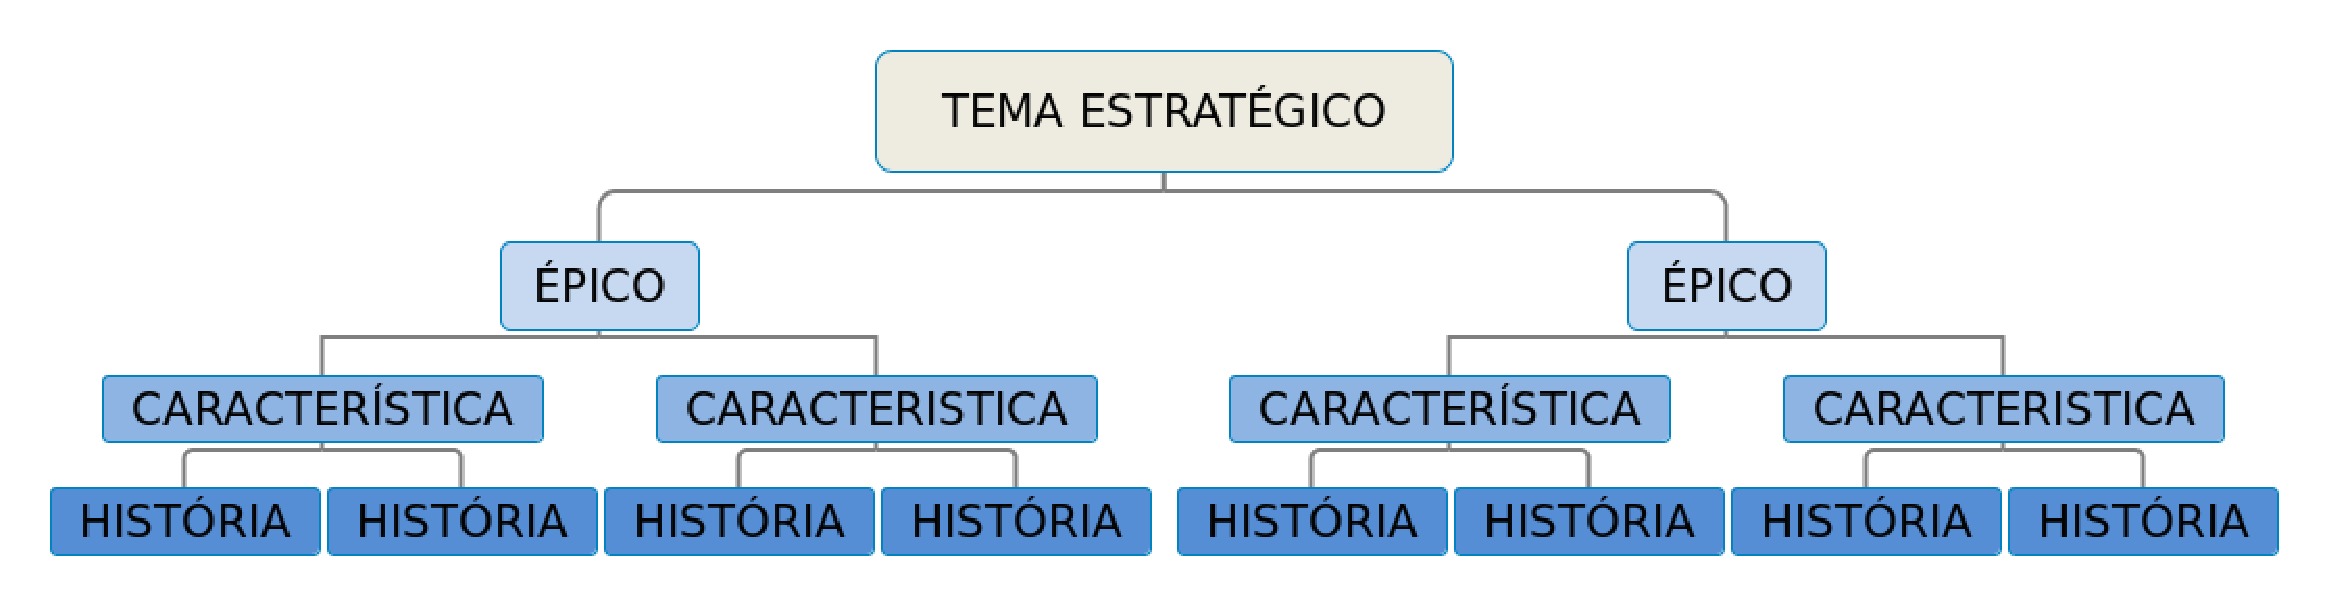
\includegraphics[keepaspectratio=true,scale=0.4]{figuras/rastreabilidade.eps}
    \label{rastreabilidade}
\end{figure}
\begin{table}[h]
    \centering
    \caption{Identificação dos requisitos em cada nível}
    \label{identificadores}
    \begin{tabular}{l|l|l|l}
        Artefato & Pré-fixo & Exemplo \\
        \hline    
        Temas estratégicos & TE & TE01, TE02, TE03 \\
        Épicos & EP & EP01, EP02 EP03 \\
        Característica & FT & FT01, FT02, FT03 \\
        Histórias & US & US01, US02, US03 \\
    \end{tabular}
\end{table}

\section{Atributos de requisitos}

Os atributos para os requisitos em qualquer um dos três níveis: portfólio, programa e time, são: 

\begin{itemize}
    \item \textbf{Identificador:} é o identificador único de cada requisito, que permite localizar e distinguir dos demais requisitos.
    \newline Ex.: TE01, EP10, FT01, US01
    \item \textbf{Descrição:} define o requisito e suas caracteristicas, assim resume o requisito em poucas palavras.
    \newline Ex.: "Cadastrar novos membros da empresa" 
    \item \textbf{Prioridade:} determina a prioridade da execução de um requisito, em geral o dono do produto, ou o responsável pelos investimentos Program Portfólio Management, Product Management que definirão a prioridade dos requisitos.
    \begin{itemize}
        \item Alta: possui um alto valor agregado para o cliente.
        \item Média: trás valor agregado ao cliente, mas não possui urgência de implementação.
        \item Baixa: o valor agredado a ser entregue para o cliente é baixo e portanto serão implementados depois dos requisitos das outras prioridades.
    \end{itemize}
    \item \textbf{Estado:} define o andamento da produção, implementação de um requisito.
    \begin{itemize}
        \item A fazer: define o requisito que não foi iniciado.
        \item Fazendo: define o estado de um requisito que foi iniciado e ainda não está concluído, independente da porcentagem de conclusão.
        \item Feito: estado para quando o requisito foi completado, ou seja, atingiu os critérios de aceitação estabelecidos.
    \end{itemize}
    \item \textbf{Pontuação:} atribui uma pontuação que caracteriza a complexidade de um requisito. No SAFe, a recomendaçao é utilizar uma adaptação dos números de Fibonacci para a pontuação (1, 2, 3, 5, 8, 13, 20, 40, 100), que leva em consideração também, o esforço do time para realizar tal tarefa \cite{safe}.
    \item \textbf{Versão:} determina qual é a versão do requisito e qual é a última versão.
    \item \textbf{Requisito de origem:} este campo é para identificar o requisito originário deste, permitindo a rastreabilidade vertical.
\end{itemize}

Exemplo:

\begin{table}[h]
\centering
\caption{Tabela de atributos}
\label{atributos}
    \begin{tabular}{l|l|l|l|r|r|l}
    Identificador & Descrição & Prioridade & Estado & Pontos & Versão & Origem \\
    \hline
    US02 & Uma breve descrição. & Alta & Fazendo & 5 & 1.0 & FT02\\
    US03 & Uma breve descrição. & Alta & A fazer & 3 & 1.0 & FT02\\
    US04 & Uma breve descrição. & Alta & A fazer  & 8 & 1.0 & FT02\\
    US05 & Uma breve descrição. & Alta & Feito  & 3 & 1.2 & FT02
    \end{tabular}
\end{table}

